\PassOptionsToPackage{unicode=true}{hyperref} % options for packages loaded elsewhere
\PassOptionsToPackage{hyphens}{url}
%
\documentclass[]{article}
\usepackage{lmodern}
\usepackage{amssymb,amsmath}
\usepackage{ifxetex,ifluatex}
\usepackage{fixltx2e} % provides \textsubscript
\ifnum 0\ifxetex 1\fi\ifluatex 1\fi=0 % if pdftex
  \usepackage[T1]{fontenc}
  \usepackage[utf8]{inputenc}
  \usepackage{textcomp} % provides euro and other symbols
\else % if luatex or xelatex
  \usepackage{unicode-math}
  \defaultfontfeatures{Ligatures=TeX,Scale=MatchLowercase}
\fi
% use upquote if available, for straight quotes in verbatim environments
\IfFileExists{upquote.sty}{\usepackage{upquote}}{}
% use microtype if available
\IfFileExists{microtype.sty}{%
\usepackage[]{microtype}
\UseMicrotypeSet[protrusion]{basicmath} % disable protrusion for tt fonts
}{}
\IfFileExists{parskip.sty}{%
\usepackage{parskip}
}{% else
\setlength{\parindent}{0pt}
\setlength{\parskip}{6pt plus 2pt minus 1pt}
}
\usepackage{hyperref}
\hypersetup{
            pdftitle={The Method of Monte Carlo},
            pdfauthor={Dr Thiyanga S Talagala},
            pdfborder={0 0 0},
            breaklinks=true}
\urlstyle{same}  % don't use monospace font for urls
\usepackage[margin=1in]{geometry}
\usepackage{color}
\usepackage{fancyvrb}
\newcommand{\VerbBar}{|}
\newcommand{\VERB}{\Verb[commandchars=\\\{\}]}
\DefineVerbatimEnvironment{Highlighting}{Verbatim}{commandchars=\\\{\}}
% Add ',fontsize=\small' for more characters per line
\usepackage{framed}
\definecolor{shadecolor}{RGB}{248,248,248}
\newenvironment{Shaded}{\begin{snugshade}}{\end{snugshade}}
\newcommand{\AlertTok}[1]{\textcolor[rgb]{0.94,0.16,0.16}{#1}}
\newcommand{\AnnotationTok}[1]{\textcolor[rgb]{0.56,0.35,0.01}{\textbf{\textit{#1}}}}
\newcommand{\AttributeTok}[1]{\textcolor[rgb]{0.77,0.63,0.00}{#1}}
\newcommand{\BaseNTok}[1]{\textcolor[rgb]{0.00,0.00,0.81}{#1}}
\newcommand{\BuiltInTok}[1]{#1}
\newcommand{\CharTok}[1]{\textcolor[rgb]{0.31,0.60,0.02}{#1}}
\newcommand{\CommentTok}[1]{\textcolor[rgb]{0.56,0.35,0.01}{\textit{#1}}}
\newcommand{\CommentVarTok}[1]{\textcolor[rgb]{0.56,0.35,0.01}{\textbf{\textit{#1}}}}
\newcommand{\ConstantTok}[1]{\textcolor[rgb]{0.00,0.00,0.00}{#1}}
\newcommand{\ControlFlowTok}[1]{\textcolor[rgb]{0.13,0.29,0.53}{\textbf{#1}}}
\newcommand{\DataTypeTok}[1]{\textcolor[rgb]{0.13,0.29,0.53}{#1}}
\newcommand{\DecValTok}[1]{\textcolor[rgb]{0.00,0.00,0.81}{#1}}
\newcommand{\DocumentationTok}[1]{\textcolor[rgb]{0.56,0.35,0.01}{\textbf{\textit{#1}}}}
\newcommand{\ErrorTok}[1]{\textcolor[rgb]{0.64,0.00,0.00}{\textbf{#1}}}
\newcommand{\ExtensionTok}[1]{#1}
\newcommand{\FloatTok}[1]{\textcolor[rgb]{0.00,0.00,0.81}{#1}}
\newcommand{\FunctionTok}[1]{\textcolor[rgb]{0.00,0.00,0.00}{#1}}
\newcommand{\ImportTok}[1]{#1}
\newcommand{\InformationTok}[1]{\textcolor[rgb]{0.56,0.35,0.01}{\textbf{\textit{#1}}}}
\newcommand{\KeywordTok}[1]{\textcolor[rgb]{0.13,0.29,0.53}{\textbf{#1}}}
\newcommand{\NormalTok}[1]{#1}
\newcommand{\OperatorTok}[1]{\textcolor[rgb]{0.81,0.36,0.00}{\textbf{#1}}}
\newcommand{\OtherTok}[1]{\textcolor[rgb]{0.56,0.35,0.01}{#1}}
\newcommand{\PreprocessorTok}[1]{\textcolor[rgb]{0.56,0.35,0.01}{\textit{#1}}}
\newcommand{\RegionMarkerTok}[1]{#1}
\newcommand{\SpecialCharTok}[1]{\textcolor[rgb]{0.00,0.00,0.00}{#1}}
\newcommand{\SpecialStringTok}[1]{\textcolor[rgb]{0.31,0.60,0.02}{#1}}
\newcommand{\StringTok}[1]{\textcolor[rgb]{0.31,0.60,0.02}{#1}}
\newcommand{\VariableTok}[1]{\textcolor[rgb]{0.00,0.00,0.00}{#1}}
\newcommand{\VerbatimStringTok}[1]{\textcolor[rgb]{0.31,0.60,0.02}{#1}}
\newcommand{\WarningTok}[1]{\textcolor[rgb]{0.56,0.35,0.01}{\textbf{\textit{#1}}}}
\usepackage{graphicx,grffile}
\makeatletter
\def\maxwidth{\ifdim\Gin@nat@width>\linewidth\linewidth\else\Gin@nat@width\fi}
\def\maxheight{\ifdim\Gin@nat@height>\textheight\textheight\else\Gin@nat@height\fi}
\makeatother
% Scale images if necessary, so that they will not overflow the page
% margins by default, and it is still possible to overwrite the defaults
% using explicit options in \includegraphics[width, height, ...]{}
\setkeys{Gin}{width=\maxwidth,height=\maxheight,keepaspectratio}
\setlength{\emergencystretch}{3em}  % prevent overfull lines
\providecommand{\tightlist}{%
  \setlength{\itemsep}{0pt}\setlength{\parskip}{0pt}}
\setcounter{secnumdepth}{0}
% Redefines (sub)paragraphs to behave more like sections
\ifx\paragraph\undefined\else
\let\oldparagraph\paragraph
\renewcommand{\paragraph}[1]{\oldparagraph{#1}\mbox{}}
\fi
\ifx\subparagraph\undefined\else
\let\oldsubparagraph\subparagraph
\renewcommand{\subparagraph}[1]{\oldsubparagraph{#1}\mbox{}}
\fi

% set default figure placement to htbp
\makeatletter
\def\fps@figure{htbp}
\makeatother

\usepackage{etoolbox}
\makeatletter
\providecommand{\subtitle}[1]{% add subtitle to \maketitle
  \apptocmd{\@title}{\par {\large #1 \par}}{}{}
}
\makeatother

\title{The Method of Monte Carlo}
\providecommand{\subtitle}[1]{}
\subtitle{STA 326 2.0 Programming and Data Analysis with R}
\author{Dr Thiyanga S Talagala}
\date{}

\begin{document}
\maketitle

{
\setcounter{tocdepth}{3}
\tableofcontents
}
\newpage

\hypertarget{introduction}{%
\section{1. Introduction}\label{introduction}}

The basics of a Monte Carlo simulation are simply to model your problem,
and than randomly simulate it until you get an answer. The best way to
understand is to go through a bunch of examples, so let's go!

\hypertarget{applications}{%
\section{2. Applications}\label{applications}}

\hypertarget{estimate-area}{%
\subsection{2.1 Estimate Area}\label{estimate-area}}

\hypertarget{example-2.1.2-estimate-area}{%
\subsubsection{Example 2.1.2 Estimate
area}\label{example-2.1.2-estimate-area}}

Then we want to find the integral from 3 to 6 \[\int_^6 \fracdx \]as
visualized below

\hypertarget{example-2.1.2-approximating-pi-3.14616}{%
\subsubsection{Example 2.1.2: Approximating Pi =
3.14616}\label{example-2.1.2-approximating-pi-3.14616}}

\[\frac{A_{circle}}{A_{square}}=\frac{\pi r^2}{4r^2}\] Equation of the
unit circle center around 0: \(x^2+y^2=r^2\)

\begin{Shaded}
\begin{Highlighting}[]
\KeywordTok{library}\NormalTok{(tidyverse)}
\NormalTok{x <-}\StringTok{ }\KeywordTok{runif}\NormalTok{(}\DecValTok{10000}\NormalTok{, }\DecValTok{-1}\NormalTok{, }\DecValTok{1}\NormalTok{)}
\NormalTok{y <-}\StringTok{ }\KeywordTok{runif}\NormalTok{(}\DecValTok{10000}\NormalTok{, }\DecValTok{-1}\NormalTok{, }\DecValTok{1}\NormalTok{)}
\NormalTok{fx <-}\StringTok{ }\NormalTok{x}\OperatorTok{^}\DecValTok{2} \OperatorTok{+}\StringTok{ }\NormalTok{y}\OperatorTok{^}\DecValTok{2}
\NormalTok{coly <-}\StringTok{  }\KeywordTok{ifelse}\NormalTok{(fx }\OperatorTok{<=}\StringTok{ }\DecValTok{1}\NormalTok{, }\DecValTok{1}\NormalTok{, }\DecValTok{0}\NormalTok{)}
\NormalTok{coly <-}\StringTok{ }\KeywordTok{as.factor}\NormalTok{(coly)}
\NormalTok{pidf <-}\StringTok{ }\KeywordTok{data.frame}\NormalTok{(}\DataTypeTok{x=}\NormalTok{x, }\DataTypeTok{y=}\NormalTok{y, }\DataTypeTok{coly=}\NormalTok{coly)}
\end{Highlighting}
\end{Shaded}

\begin{Shaded}
\begin{Highlighting}[]
\CommentTok{# without coord_equal()}
\KeywordTok{ggplot}\NormalTok{(pidf, }\KeywordTok{aes}\NormalTok{(}\DataTypeTok{x=}\NormalTok{x, }\DataTypeTok{y=}\NormalTok{y, }\DataTypeTok{col=}\NormalTok{coly)) }\OperatorTok{+}\StringTok{ }\KeywordTok{geom_point}\NormalTok{()  }\OperatorTok{+}
\StringTok{   }\KeywordTok{scale_colour_manual}\NormalTok{(}\DataTypeTok{values =} \KeywordTok{c}\NormalTok{(}\StringTok{"#e7298a"}\NormalTok{, }\StringTok{"#1b9e77"}\NormalTok{))}
\end{Highlighting}
\end{Shaded}

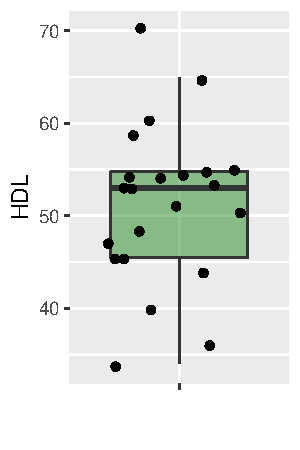
\includegraphics{Monte_Carlo_files/figure-latex/unnamed-chunk-3-1.pdf}

\begin{Shaded}
\begin{Highlighting}[]
\CommentTok{# with coord_equal()}
\KeywordTok{ggplot}\NormalTok{(pidf, }\KeywordTok{aes}\NormalTok{(}\DataTypeTok{x=}\NormalTok{x, }\DataTypeTok{y=}\NormalTok{y, }\DataTypeTok{col=}\NormalTok{coly)) }\OperatorTok{+}\StringTok{ }\KeywordTok{geom_point}\NormalTok{() }\OperatorTok{+}
\StringTok{   }\KeywordTok{scale_colour_manual}\NormalTok{(}\DataTypeTok{values =} \KeywordTok{c}\NormalTok{(}\StringTok{"#e7298a"}\NormalTok{, }\StringTok{"#1b9e77"}\NormalTok{)) }\OperatorTok{+}\StringTok{ }
\StringTok{  }\KeywordTok{coord_equal}\NormalTok{()}
\end{Highlighting}
\end{Shaded}

\includegraphics{Monte_Carlo_files/figure-latex/unnamed-chunk-3-2.pdf}

\begin{Shaded}
\begin{Highlighting}[]
\NormalTok{compute_pi_mc_sim <-}\StringTok{ }\ControlFlowTok{function}\NormalTok{(n)\{}
\NormalTok{  x <-}\StringTok{ }\KeywordTok{runif}\NormalTok{(n, }\DecValTok{-1}\NormalTok{, }\DecValTok{1}\NormalTok{)}
\NormalTok{  y <-}\StringTok{ }\KeywordTok{runif}\NormalTok{(n, }\DecValTok{-1}\NormalTok{, }\DecValTok{1}\NormalTok{)}
\NormalTok{  count <-}\StringTok{ }\DecValTok{0}
  \ControlFlowTok{for}\NormalTok{(i }\ControlFlowTok{in} \DecValTok{1}\OperatorTok{:}\NormalTok{n)\{}
    \ControlFlowTok{if}\NormalTok{(x[i]}\OperatorTok{^}\DecValTok{2} \OperatorTok{+}\StringTok{ }\NormalTok{y[i]}\OperatorTok{^}\DecValTok{2} \OperatorTok{<}\StringTok{ }\DecValTok{1} \OperatorTok{|}\StringTok{ }\NormalTok{x[i]}\OperatorTok{^}\DecValTok{2} \OperatorTok{+}\StringTok{ }\NormalTok{y[i]}\OperatorTok{^}\DecValTok{2} \OperatorTok{==}\StringTok{ }\DecValTok{1}\NormalTok{)\{}
\NormalTok{      count =}\StringTok{ }\NormalTok{count }\OperatorTok{+}\StringTok{ }\DecValTok{1}
      
\NormalTok{    \} }\ControlFlowTok{else}\NormalTok{ \{}
\NormalTok{      count}
\NormalTok{    \}}
    
\NormalTok{  \}}
  
\NormalTok{ pi <-}\StringTok{ }\NormalTok{(count}\OperatorTok{/}\NormalTok{n) }\OperatorTok{*}\StringTok{ }\DecValTok{4}
\NormalTok{ pi}
 
\NormalTok{\}}
\KeywordTok{compute_pi_mc_sim}\NormalTok{(}\DecValTok{100}\NormalTok{)}
\end{Highlighting}
\end{Shaded}

\begin{verbatim}
[1] 3.04
\end{verbatim}

\begin{Shaded}
\begin{Highlighting}[]
\KeywordTok{compute_pi_mc_sim}\NormalTok{(}\DecValTok{1000}\NormalTok{)}
\end{Highlighting}
\end{Shaded}

\begin{verbatim}
[1] 3.18
\end{verbatim}

\begin{Shaded}
\begin{Highlighting}[]
\KeywordTok{compute_pi_mc_sim}\NormalTok{(}\DecValTok{10000}\NormalTok{)}
\end{Highlighting}
\end{Shaded}

\begin{verbatim}
[1] 3.1288
\end{verbatim}

Write a function to approximate \(\pi\) using Monte Carlo simulations.

\hypertarget{example-2.1.2-your-turn}{%
\subsubsection{Example 2.1.2: YOUR TURN}\label{example-2.1.2-your-turn}}

Estimate area under the curve withing \(x \in [0, 1]\) using Monte Carlo
simulation approach.

\(f(x) = sin(10x)^{2sin(x)}x+0.1\)

\begin{Shaded}
\begin{Highlighting}[]
\NormalTok{x1 <-}\StringTok{ }\KeywordTok{seq}\NormalTok{(}\DecValTok{0}\NormalTok{, }\DecValTok{1}\NormalTok{, }\FloatTok{0.01}\NormalTok{)}
\NormalTok{f1 <-}\StringTok{ }\NormalTok{((}\KeywordTok{sin}\NormalTok{(}\DecValTok{10}\OperatorTok{*}\NormalTok{x1}\OperatorTok{^}\DecValTok{2}\NormalTok{))}\OperatorTok{^}\DecValTok{2}\OperatorTok{*}\KeywordTok{sin}\NormalTok{(x1))}\OperatorTok{*}\NormalTok{x1}\FloatTok{+0.1}
\NormalTok{df1 <-}\StringTok{ }\KeywordTok{data.frame}\NormalTok{(}\DataTypeTok{x=}\NormalTok{x1, }\DataTypeTok{y=}\NormalTok{f1)}
\KeywordTok{ggplot}\NormalTok{(df1, }\KeywordTok{aes}\NormalTok{(}\DataTypeTok{x=}\NormalTok{x1, }\DataTypeTok{y=}\NormalTok{f1))}\OperatorTok{+}\KeywordTok{geom_line}\NormalTok{() }\OperatorTok{+}\StringTok{ }\KeywordTok{coord_equal}\NormalTok{()}
\end{Highlighting}
\end{Shaded}

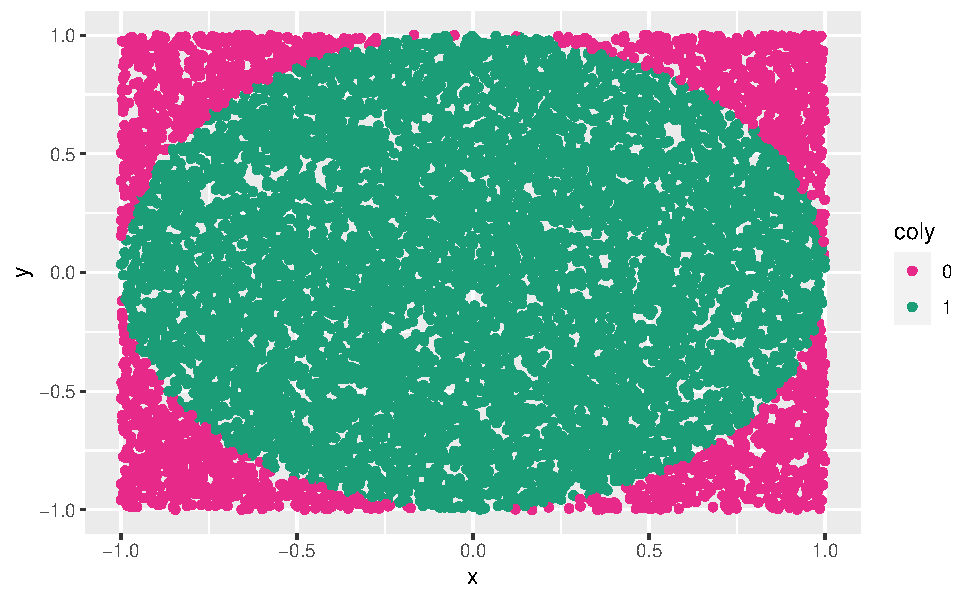
\includegraphics{Monte_Carlo_files/figure-latex/unnamed-chunk-5-1.pdf}

\begin{Shaded}
\begin{Highlighting}[]
\KeywordTok{set.seed}\NormalTok{(}\DecValTok{2020}\NormalTok{)}
\NormalTok{x =}\StringTok{ }\KeywordTok{runif}\NormalTok{(}\DecValTok{10000}\NormalTok{, }\DataTypeTok{min =}\DecValTok{0}\NormalTok{ , }\DataTypeTok{max =}\DecValTok{1}\NormalTok{ )}
\NormalTok{y =}\StringTok{ }\KeywordTok{runif}\NormalTok{(}\DecValTok{10000}\NormalTok{, }\DataTypeTok{min =}\DecValTok{0}\NormalTok{ , }\DataTypeTok{max =}\DecValTok{1}\NormalTok{ )}
\NormalTok{fx <-}\StringTok{ }\NormalTok{((}\KeywordTok{sin}\NormalTok{(}\DecValTok{10}\OperatorTok{*}\NormalTok{x}\OperatorTok{^}\DecValTok{2}\NormalTok{))}\OperatorTok{^}\DecValTok{2}\OperatorTok{*}\KeywordTok{sin}\NormalTok{(x))}\OperatorTok{*}\NormalTok{x}\FloatTok{+0.1}
\NormalTok{coly <-}\StringTok{  }\KeywordTok{ifelse}\NormalTok{(y }\OperatorTok{<}\StringTok{ }\NormalTok{fx, }\DecValTok{1}\NormalTok{, }\DecValTok{0}\NormalTok{)}
\NormalTok{coly <-}\StringTok{ }\KeywordTok{as.factor}\NormalTok{(coly)}
\NormalTok{df2 <-}\StringTok{ }\KeywordTok{data.frame}\NormalTok{(}\DataTypeTok{x=}\NormalTok{x, }\DataTypeTok{y=}\NormalTok{y, }\DataTypeTok{coly=}\NormalTok{coly)}
\KeywordTok{ggplot}\NormalTok{(df2, }\KeywordTok{aes}\NormalTok{(}\DataTypeTok{x=}\NormalTok{x, }\DataTypeTok{y=}\NormalTok{y, }\DataTypeTok{col=}\NormalTok{coly)) }\OperatorTok{+}\StringTok{ }\KeywordTok{geom_point}\NormalTok{() }\OperatorTok{+}\StringTok{   }\KeywordTok{scale_colour_manual}\NormalTok{(}\DataTypeTok{values =} \KeywordTok{c}\NormalTok{(}\StringTok{"#e7298a"}\NormalTok{, }\StringTok{"#1b9e77"}\NormalTok{)) }\OperatorTok{+}\StringTok{ }\KeywordTok{coord_equal}\NormalTok{()}
\end{Highlighting}
\end{Shaded}

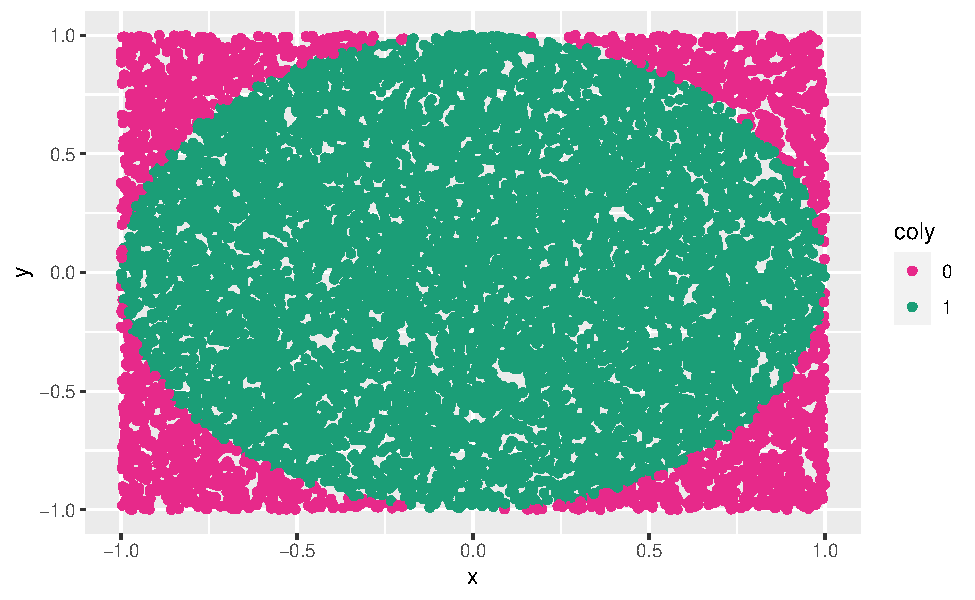
\includegraphics{Monte_Carlo_files/figure-latex/unnamed-chunk-6-1.pdf}

\hypertarget{monte-carlo-integration}{%
\subsection{2.2 Monte Carlo Integration}\label{monte-carlo-integration}}

Suppose we want to calculate the integral \(\int_a^bg(x)dx\) for a
continuous function \(g\) over the closed and bounded interval {[}a,
b{]}. If the anti-derivative of \(g\) does not exist, then numerical
integration is in order. A simple numerical technique is the method of
Monte Carlo. We can write the integral as

\[\int_a^bg(x)dx=(b-a)\int_a^b\frac{1}{a-b}dx=(b-a)E[g(X)],\]

where \(X\) has the \(uniform(a, b)\) distribution.

To compute the estimated value first a set of random numbers
\(X_1, X_2, X_n\) of size \(n\) is, then compute \(Y_i = (b-a)g(X_i)\).
Then \(\bar{Y}\) is a consistent estimate of \(\int_a^bg(x)dx\).

\hypertarget{example-2.2.1-approximating-pi-using-monte-carlo-integration.}{%
\subsubsection{Example 2.2.1: Approximating Pi using Monte Carlo
Integration.}\label{example-2.2.1-approximating-pi-using-monte-carlo-integration.}}

Let \(g(x)=4\sqrt{1-x^2}\) for \(0 < x < 1\). Then,

\[\pi = \int_0^1g(x)dx = E[g(X)],\]

where \(X\) has the \(uniform(0, 1)\) distribution.

Write an R function to obtain point estimate and 95\% confidence
interval for \(pi\) using the sample sizes, 100, 1000, 10000 , 100000
and fill the blanks in the following table.

\begin{Shaded}
\begin{Highlighting}[]
\NormalTok{pi_mi <-}\StringTok{ }\ControlFlowTok{function}\NormalTok{(n)\{}
  
\NormalTok{  random.uniform <-}\StringTok{ }\KeywordTok{runif}\NormalTok{(n)}
\NormalTok{  sample_gx_values <-}\StringTok{ }\DecValTok{4}\OperatorTok{*}\KeywordTok{sqrt}\NormalTok{(}\DecValTok{1}\OperatorTok{-}\NormalTok{random.uniform}\OperatorTok{^}\DecValTok{2}\NormalTok{)}
  \CommentTok{# point estimate}
\NormalTok{  y_bar <-}\StringTok{ }\KeywordTok{mean}\NormalTok{(sample_gx_values)}
  \CommentTok{# standard error}
\NormalTok{  se <-}\StringTok{ }\KeywordTok{sqrt}\NormalTok{(}\KeywordTok{var}\NormalTok{(sample_gx_values)}\OperatorTok{/}\NormalTok{n)}
  \CommentTok{# 95% confidence interval}
\NormalTok{  interval_estimate_lower <-}\StringTok{ }\NormalTok{y_bar }\OperatorTok{-}\StringTok{ }\NormalTok{(}\FloatTok{1.96} \OperatorTok{*}\StringTok{ }\NormalTok{se)}
\NormalTok{  interval_estimate_upper <-}\StringTok{ }\NormalTok{y_bar }\OperatorTok{+}\StringTok{ }\NormalTok{(}\FloatTok{1.96} \OperatorTok{*}\StringTok{ }\NormalTok{se)}
  \CommentTok{#output}
\NormalTok{  tibble}\OperatorTok{::}\KeywordTok{tibble}\NormalTok{(}\DataTypeTok{pi=}\NormalTok{y_bar, }
                 \DataTypeTok{CI.lower=}\NormalTok{interval_estimate_lower,  }
                 \DataTypeTok{CI.upper=}\NormalTok{interval_estimate_upper)}
  
\NormalTok{\}}

\KeywordTok{pi_mi}\NormalTok{(}\DecValTok{100}\NormalTok{)}
\end{Highlighting}
\end{Shaded}

\begin{verbatim}
# A tibble: 1 x 3
     pi CI.lower CI.upper
  <dbl>    <dbl>    <dbl>
1  2.97     2.78     3.16
\end{verbatim}

\begin{Shaded}
\begin{Highlighting}[]
\KeywordTok{pi_mi}\NormalTok{(}\DecValTok{1000}\NormalTok{)}
\end{Highlighting}
\end{Shaded}

\begin{verbatim}
# A tibble: 1 x 3
     pi CI.lower CI.upper
  <dbl>    <dbl>    <dbl>
1  3.15     3.10     3.21
\end{verbatim}

\begin{Shaded}
\begin{Highlighting}[]
\KeywordTok{pi_mi}\NormalTok{(}\DecValTok{10000}\NormalTok{)}
\end{Highlighting}
\end{Shaded}

\begin{verbatim}
# A tibble: 1 x 3
     pi CI.lower CI.upper
  <dbl>    <dbl>    <dbl>
1  3.14     3.12     3.15
\end{verbatim}

\begin{Shaded}
\begin{Highlighting}[]
\KeywordTok{pi_mi}\NormalTok{(}\DecValTok{100000}\NormalTok{)}
\end{Highlighting}
\end{Shaded}

\begin{verbatim}
# A tibble: 1 x 3
     pi CI.lower CI.upper
  <dbl>    <dbl>    <dbl>
1  3.15     3.14     3.15
\end{verbatim}

YOUR TURN:

\hypertarget{example-2.2.2-your-turn}{%
\subsubsection{Example 2.2.2: YOUR TURN}\label{example-2.2.2-your-turn}}

Write an R function to estimate \(log 2\) using Monte Carlo Integration
method. Obtain a point estimate, and 95\% confidence interval for
estimate using 10000 simulations and compare it to the true value.

\emph{Hint}

\(log \text{ }2 = \int_0^1\frac{1}{x+1}dx.\)

\hypertarget{example-2.2.3-your-turn}{%
\subsubsection{Example 2.2.3: YOUR TURN}\label{example-2.2.3-your-turn}}

\hypertarget{hypothesis-testing-based-on-simulations}{%
\subsection{2.3 Hypothesis testing based on
simulations}\label{hypothesis-testing-based-on-simulations}}

\textbf{Steps: }

Let N be the number of simulations.

\begin{enumerate}
\def\labelenumi{\arabic{enumi}.}
\item
  Set \(k=1\) and \(I = 0\).
\item
  Simulate a random sample of size \(n\) from the distribution X and
  compute the test statistic \(t\).
\item
  If \(\text{test statistic} > \text{critical value}\), increase \(I\)
  by 1.
\item
  Repeat the process until \(k=N\)
\item
  Calculate the p-value
\end{enumerate}

\end{document}
